\documentclass{beamer}

\usetheme{CambridgeUS}
\usepackage{graphicx}
\usepackage{caption}
\usepackage{subcaption}
\usepackage{listings}
\usepackage[style=authoryear]{biblatex}
\bibliography{hmm}

\title[HMM]{Hidden Markov Models}

\subtitle{Theoretical Aspects. Octave Implementation. Applications}

\author[A. Sorici, T. Berariu]{Alexandru Sorici, Tudor Berariu}

\institute[ARIA]{Romanian Asociation for Artificial Intelligence}

\date{October, 27$^{\text{th}}$, 2012}


%% TODO de pus frumos titlurile secțiunilor


%% Pentru a pune contents si frame cu titlu pe part
\makeatletter 
\AtBeginPart{%
\addtocontents{toc}{\protect\beamer@partintoc{\the\c@part}{\beamer@partnameshort}{\the\c@page}
  }%
  % \begin{frame}
  %   \center{ 
  %     \Large{
  %       \beamer@partname 
  %     }
  %   }
  % \end{frame}
  \begin{frame}{Outline}
    \tableofcontents[currentpart]
  \end{frame}
}


%% number, shortname, page.
\providecommand\beamer@partintoc[3]{%
  \ifnum\c@tocdepth=-1\relax
  % requesting onlyparts.
  \center{
  \makebox[20em]{PART #1.} \makebox[20em]{\Large{\textbf{#2}}}
}
  \par
  \fi } 

\define@key{beamertoc}{onlyparts}[]{%
  \c@tocdepth=-1\relax } \makeatother%


%% pentru a pune inainte de fiecare sectiune
\AtBeginSubsection[] {
  \begin{frame}{Outline}
    \tableofcontents[currentsection,currentsubsection,hideallsections]
  \end{frame}
}



\begin{document}
\maketitle

\begin{frame}
  \tableofcontents[onlyparts]
\end{frame}

\begin{frame}
  \frametitle{Outline}
  \tableofcontents[pausesections]
\end{frame}



\part{Intro}

\section{ARIA Education Workshops}
\label{sec:aria}

%% TODO: de luat de la Andreea Ciortea

\subsection{ARIA's Mission}
\label{sec:arimamis}

%% TODO: de luat de la Andreea Ciortea

\subsection{ARIA Education}
\label{sec:ae}

%% TODO: de luat de la Andreea Ciortea

\begin{frame}
  \frametitle{ARIA EDU} :)
\end{frame}

\subsection{Workshop Program}
\label{sec:program}
%% TODO: program pe ore (nu cu topics de discutat, ci mai degraba cu
%% time split)
\begin{frame}
  \frametitle{Today's Program}

  \begin{table}[h]
    \centering
    \begin{tabular}{|| l | l ||}
      \hline \hline
      9:00 & Registration \\
      \hline
      10:00 & Rahaturi despre ARIA \\
      \hline \hline
      11:00 & HMM Theory \\
      \hline \hline
      
    \end{tabular}
    % \caption{Today's Program}
    \label{tab:program}
  \end{table}
\end{frame}

\part{Theory of HMMs}


\section{Machine Learning Applications for HMM}
\label{sec:ml}

% introducere in invatare automata + categorisire probleme
\subsection{Machine Learning}
\label{sec:hmm_in_ml}

\begin{frame}
  \frametitle{What is Machine Learning?}
  \begin{block}{Machine Learning}
    A computer program is said to learn from experience $E$ with
    respect to some class of tasks $T$ and performance measure $P$, if
    its performance at tasks in $T$, as measured by $P$, improves with
    experience $E$.
  \end{block}
\end{frame}

\begin{frame}
  \frametitle{Machine Learning Applications}
  \begin{itemize}
  \item Computer Vision: Google Car
  \item Machine Translation
  \item Speech Recognition
  \item Recommender Systems
  \item Intelligent Advertising
  \end{itemize}
\end{frame}

% aplicatii specifice hmm-urilor de ce am ales hmm-urile
\subsection{Where do HMMs fit into Machine Learning?}
\label{sec:apps}

\begin{frame}
  \frametitle{Machine Learning Classification}
  Types of Machine Learning Problems
  \begin{columns}
    \column{0.7\textwidth}
    \begin{itemize}
    \item Regression
    \item Classification
    \item Reinforcement Learning
    \end{itemize}
    \begin{itemize}
    \item supervised learning (eg. ..)
    \item unsupervised
    \end{itemize}
    \column{0.3\textwidth}
    \includegraphics[width=\textwidth]{graphics/ml.pdf}
  \end{columns}
\end{frame}

%% aici facem tranzitie de la problema generala de ML
%% la probleme cu secvente temporale, markov stuff, dbn shit
%% adica HMM-uri :))

%% Markov models, Dynamic Bayesian Networks
\begin{frame}
  \frametitle{Sequence / Temporal problems (I)}
  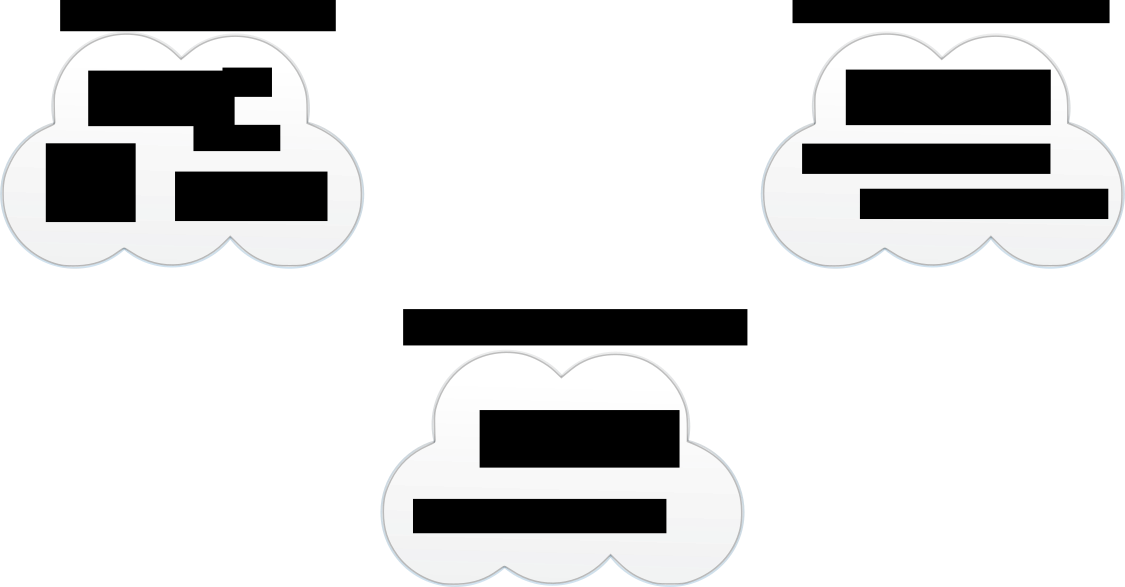
\includegraphics[width=\textwidth]{images/time_series_problems_1.pdf}
\end{frame}

\begin{frame}
  \frametitle{Sequence / Temporal problems (II)}
  \includegraphics[width=\textwidth]{images/time_series_problems_2.pdf}
  %Koller and Frideman au scris in \cite{KollerFriedman09}
  % temporal sequences
  % DBN for ts
  % HMM as a special case of DBN
\end{frame}


% descrierea a ceea ce inseamna Probabilistic Reasoning over Time (capitol 15.2 AI a modern approach)
% 	- states and observations
\begin{frame}[t]
  \frametitle{Probabilistic Reasoning over Time - Models}
	Consider some of the previously presented problems ...
	\vspace*{0.5em}
	\pause	
	
	How do we model such dynamic situations? 
	\vspace*{1em}
	\pause	
	
	\textbf{States and Observations}
	\begin{itemize}
		\item The process of change is viewed as a series of \alert{time slices (snapshots)}
		\item Each time slice contains a set of random variables
    	\begin{itemize}
	    	\item $\mathbf{O}_t$ - set of all \alert{\emph{observable}} evidence variables at time \emph{t}
			\item $\mathbf{Q}_t$ - set of all \alert{\emph{unobservable / hidden}} state variables at time \emph{t}
		\end{itemize}
	\end{itemize}
\end{frame}

%	- stationary process, Markov assumption, Sensor model
\begin{frame}[t]
  \frametitle{Probabilistic Reasoning over Time - Assumptions}
	Consider some of the previously presented problems ...
	\vspace*{0.5em}
	\pause	
	
	What \alert{assumptions} (if any) do we make?
	\pause	
	
	\begin{block}{Stationary Process}
		The process of change is governed by laws \alert{that do not themselves change over time}.\\
		\alert{Implication:} we need to specify conditional distributions only for the variables within a \emph{representative} timeslice.
	\end{block}
	
	\pause	
	
	\begin{block}{Markov Assumption}
		The current state in a process of change depends only on a \alert{finite history} of previous states.
		\\
		\alert{Implication:} there is a \alert{bounded} number of ``parents'' for the variables in each time 
		slice.\\
		$\mathbf{P}(\mathbf{Q}_t \vert \mathbf{Q}_{1:t-1}) = \mathbf{P}(\mathbf{Q}_t \vert \mathbf{Q}_{t-1})$
		\hspace*{1em}
		$\mathbf{P}(\mathbf{O}_t \vert \mathbf{Q}_{1:t}, \mathbf{Q}_{1:t-1}) = \mathbf{P}(\mathbf{O}_t \vert \mathbf{Q}_t)$
	\end{block}
  
\end{frame}

%	- inference in temporal models
%		- filtering
%		- prediction
%		- smoothing (hindsight)
%		- most likely explanation
%		- model learning
\begin{frame}
  \frametitle{Probabilistic Reasoning over Time - Inference}
	What are the basic inference tasks that must be solved?
	\pause	
	
	\begin{block}{Filtering (monitoring)}
		The task of computing the \alert{belief state} - the posterior distribution over the 
		\alert{current state}, given all evidence to date.\\
		$\mathbf{P}(\mathbf{Q}_t \vert \mathbf{o}_{1:t})$
	\end{block}
	\pause
	
	\begin{block}{Evaluation (likelihood)}
		The task of computing the \alert{likelihood} of the evidence up to present.\\
		$\mathbf{P}(\mathbf{o}_{1:t})$
	\end{block}  
\end{frame}

\begin{frame}
  \frametitle{Probabilistic Reasoning over Time - Inference}
	\begin{block}{Prediction}
		The task of computing the posterior distribution over the \alert{future state}, 
		given all evidence to date.\\
		$\mathbf{P}(\mathbf{Q}_{t+k} \vert \mathbf{o}_{1:t})$, for some $k > 0$
	\end{block}
	\pause
	
	\begin{block}{Smoothing (hindsight)}
		The task of computing the posterior distribution over a \alert{past state}, 
		given all evidence to the present.\\
		$\mathbf{P}(\mathbf{Q}_k \vert \mathbf{o}_{1:t})$, for some $1 \le k < t$\\
		Provides a better estimate of the state than was available at the time.
	\end{block}
\end{frame}

\begin{frame}
  \frametitle{Probabilistic Reasoning over Time - Inference}
	\begin{block}{Most likely explanation}
		Given a \emph{sequence of observations}, find the \alert{sequence of states} that is 
		\alert{most likely} to have generated those observations.
		$argmax_{q_{1:t}}$ $\mathbf{P}(\mathbf{q}_{t+k} \vert \mathbf{o}_{1:t})$, for some $k > 0$
	\end{block}
	\pause
	
	\begin{block}{Learning}
		Given a set of \emph{observation sequences}, find a method to learn the \alert{transition} 
		(e.g. $\mathbf{P}(\mathbf{q}_{t+1} = s_j \vert \mathbf{q}_t = s_i)$, $1 \le i,j < N$) and \alert{sensor} ($\mathbf{P}(\mathbf{o}_t \vert \mathbf{q}_t)$) 
		\alert{models} from the observations.
	\end{block}
\end{frame}

\begin{frame}[t]
    \frametitle{Probabilistic Reasoning over Time - Known Methods}
    
  	\begin{block}{Dynamic Bayesian Networks (DBN)}
  		A DBN is Bayesian network that represents a temporal probability model.
  	\end{block}
  	
  	\begin{figure}
  		\centering
  		
		\begin{subfigure}[b]{0.18\textwidth}
			\centering
  			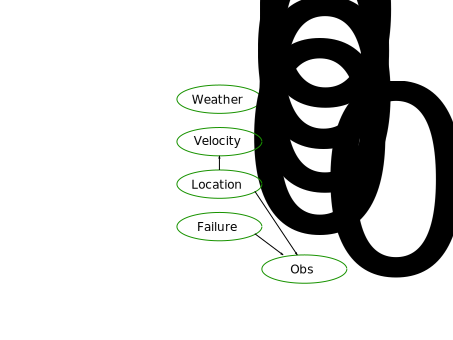
\includegraphics[width=\textwidth]{dbn-vehicle/zero.pdf}
  			\caption{\tiny{the 2-time-slice Bayesian Network}}
  			\label{fig:2TBN}
  		\end{subfigure}
  		\begin{subfigure}[b]{0.33\textwidth}
			\centering
			\includegraphics[width=\textwidth]{dbn-vehicle/transition.pdf}
  			\caption{\tiny{the time 0 network}}
  			\label{fig:zeroDBN}
  		\end{subfigure}
  		\begin{subfigure}[b]{0.39\textwidth}
			\centering
			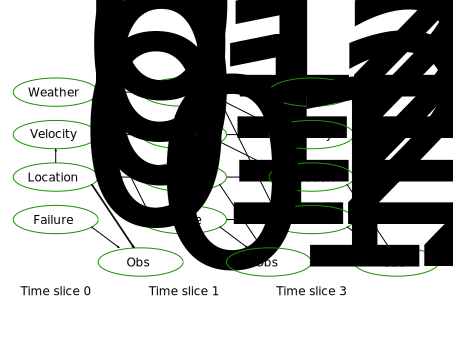
\includegraphics[width=\textwidth]{dbn-vehicle/unrolled.pdf} 
  			\caption{\tiny{unrolled DBN over 3 time slices}}
  			\label{fig:unrolledDBN}
  		\end{subfigure}
  		\caption{\tiny{A highly simplified DBN for monitoring a vehicle \parencite{KollerFriedman09}}}
  		\label{fig:DBN}
  	\end{figure}
  	
  	Applied in problems like: object tracking, human activity recognition, protein sequencing etc.
\end{frame}


\begin{frame}[t]
    \frametitle{Probabilistic Reasoning over Time - Known Methods}
  
  \begin{block}{Kalman Filters (Linear Dynamical Systems)}
  	A temporal model of one or more real-valued variables that \alert{evolve linearly} over time, with some 
  	\alert{Gaussian noise}.
  \end{block}
  
  \begin{columns}[T]
  	\column{0.4\textwidth}
  	\begin{figure}
  		\centering
  		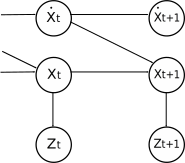
\includegraphics[height=0.35\textheight]{images/kalman_filter_simple.pdf}
  		\caption{\tiny{BN structure for a linear dynamical system with position $X_t$, 
  		velocity $\dot{X}_t$, and position measurement $Z_t$}}
  	\end{figure}
	  
  	\column{0.6\textwidth}
  	\begin{itemize}
  	\item \footnotesize{can be viewed as DBNs where all variables are continuous and all dependencies are 
  		linear gaussian}
  	\item \footnotesize{wide application in \textbf{object tracking}}
  \end{itemize}
  \end{columns}
  
\end{frame}

\begin{frame}[t]
    \frametitle{Probabilistic Reasoning over Time - Known Methods}
  
  \begin{block}{Hidden Markov Models (HMM)}
  	An HMM is a temporal probabilistic model in which the state of the process is described by 
  	\alert{a single discrete} random variable. The possible values of the variable are the possible states of the world.
  \end{block}
  
  \vspace*{1em}
  
  Used successfully in applications like:
  \begin{itemize}
  	\item Handwriting Recognition
  	\item Gesture Recognition
  	\item Speech Recognition
  	\item Part-of-Speech Tagging
  	\item DNA Sequencing
  \end{itemize}
\end{frame}


\section{Theory of HMMs}
\label{sec:theory}

\subsection{The 3 things you want from an HMM}
\label{sec:problems}

\begin{frame}
  
  The 3 fundamental problems \parencite{rabiner1989tutorial}
  \begin{itemize}
  	\item Particularization of temporal inference problems to the HMM case
  	\item The restricted structure of the HMM allows for elegant implementations of all the basic algorithms
  \end{itemize}
  \pause

  \begin{block}{Evaluation Problem}
    Given a model and a sequence of observations, how do we compute the probability that the \alert{observed 
    sequence} was produced by the model?
  \end{block}
  \pause
  \begin{block}{Best Explanation of Observations Problem}
    Given a model and a sequence of observations how do we choose a corresponding sequence of \alert{states} which 
    \emph{gives meaning} to the observations? How do we \emph{uncover} the hidden part of the model?
  \end{block}
  \pause
  \begin{block}{Model Estimation (Training) Problem}
    Given some observed sequences, how do we adjust the \alert{parameters} of an HMM model that best tries to explain 
    the observations? 
    
  \end{block}

\end{frame}


\subsection{Mathematical Foundations for HMMs}
\label{sec:math}


\begin{frame}
  \frametitle{An example problem: Emotional states}
  \begin{columns}[T]
    \column{0.58\textwidth}
    \only<1>{\framebox{\includegraphics[width=\textwidth]{graphics/example/hmm-final-m.pdf}}}
    \only<2>{\framebox{\includegraphics[width=\textwidth]{graphics/example/hmm-final-n.pdf}}}
    \only<3>{\framebox{\includegraphics[width=\textwidth]{graphics/example/hmm-final-o.pdf}}}
    \only<4>{\framebox{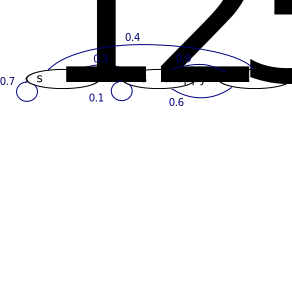
\includegraphics[width=\textwidth]{graphics/example/hmm-final-q.pdf}}}
    \only<5>{\framebox{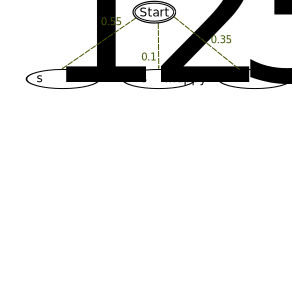
\includegraphics[width=\textwidth]{graphics/example/hmm-final-r.pdf}}}
    \only<6>{\framebox{\includegraphics[width=\textwidth]{graphics/example/hmm-final-s.pdf}}}
    \only<7>{\framebox{\includegraphics[width=\textwidth]{graphics/example/hmm-final-t.pdf}}}
    \only<8>{\framebox{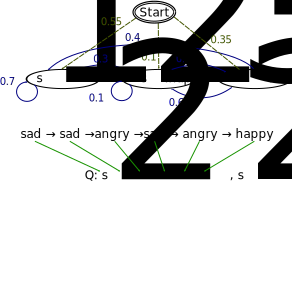
\includegraphics[width=\textwidth]{graphics/example/hmm-final-u.pdf}}}
    \only<9>{\framebox{\includegraphics[width=\textwidth]{graphics/example/hmm-final-v.pdf}}}
    \only<10>{\framebox{\includegraphics[width=\textwidth]{graphics/example/hmm-final-v2.pdf}}}
    \only<11-12>{\framebox{\includegraphics[width=\textwidth]{graphics/example/hmm-final-w.pdf}}}
    \only<13>{\framebox{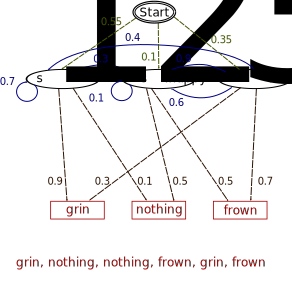
\includegraphics[width=\textwidth]{graphics/example/hmm-final-x.pdf}}}
    \only<14>{\framebox{\includegraphics[width=\textwidth]{graphics/example/hmm-final-y.pdf}}}
    \only<15>{\framebox{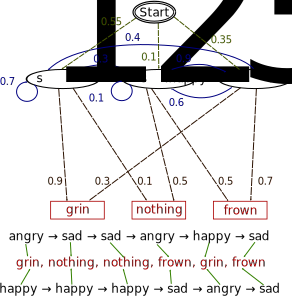
\includegraphics[width=\textwidth]{graphics/example/hmm-final-z.pdf}}}
    \only<16> {
      \begin{itemize}
      \item Example inspired from: \\\vspace*{1em}
        \fullcite{zubek2006introduction}
      \end{itemize}

    }
    

    \column{0.4\textwidth} \only<1>{ Let's consider a simple example:
      \\ \ a robot that tracks the emotional states of a player.  }
    \only<2>{ $\mathbf{N}$ - number of states \\ \vspace*{.5em}
      $\mathbf{N}=3$ \\ \vspace*{.5em} states:
      \begin{itemize}
      \item $s_1$: happy
      \item $s_2$: sad
      \item $s_3$: angry
      \end{itemize}

    }\only<3-4> { $\mathbf{A}$ - state transition probability
      distribution \\ \vspace*{.5em} \small{ $\mathbf{A} = \lbrace
        a_{i,j} \rbrace, \: 1 \le i, j \le N$ \\ \vspace*{.5em}
        $a_{i,j} = P(q_{t+1}=s_j \vert q_t = s_i)$
        \begin{itemize}
        \item $a_{\mathbf{1},1} = 0.7$
        \item $a_{\mathbf{1},2} = 0.3$
        \item $a_{\mathbf{1},3} = 0$
        \end{itemize}
        $\displaystyle\sum_{j=1}^{N}a_{i,j}=1, \quad 1 \le i \le N$ }
      \visible<4-> { $\mathbf{A} = \bordermatrix{~ & s_1 & s_2 & s_3
          \cr s_1 & 0.7 & 0.3 & 0 \cr s_2 & 0 & 0.9 & 0.1 \cr s_3 &
          0.4 & 0.6 & 0 \cr}$ }

    }
    
    \only<5>{ $\mathbf{\Pi}$ - initial state distribution \\
      \vspace*{0.5em} $\mathbf{\Pi} = \lbrace \pi_i \rbrace,\quad 1
      \le i \le N$ \\ \vspace*{0.5em} $\pi_i = P(q_1 = s_i)$ \\
      \vspace*{0.5em}
      
      $ \mathbf{\Pi} = \bordermatrix{ ~ & s_1 & s_2 & s_3 \cr ~ & 0.35
        & 0.1 & 0.55 \cr} $ }
    
    \only<6-8>{ $A = \bordermatrix{~ & s_1 & s_2 & s_3 \cr s_1 & 0.7 &
        0.3 & 0 \cr s_2 & 0 & 0.9 & 0.1 \cr s_3 & 0.4 & 0.6 & 0 \cr}$
      \\ \vspace*{0.25em} $\Pi = \bordermatrix{ ~ & s_1 & s_2 & s_3
        \cr ~ & 0.35 & 0.1 & 0.55 \cr}$ \\ \vspace*{0.25em}
      \visible<8> { $Q = [ q_1 q_2 \cdots q_T ]$ \small{
          \begin{equation*}
            \begin{split}
              P(Q & \vert A,\Pi)= \\ & = \pi_{q_1}a_{q_1,q_2}\cdots
              a_{q_{T-1},q_T}
            \end{split}
          \end{equation*}
          \begin{equation*}
            \begin{split}
              P(s_2,s_2,s_3,s_2,s_3,s_1\vert A,\Pi) = \\
              = \pi_2 \cdot a_{2,2} \cdot a_{2,3} \cdot a_{3,2} \cdot a_{2,3} \cdot a_{3,1} \\
              = \scriptstyle{0.1 \cdot 0.3 \cdot 0.1 \cdot 0.9 \cdot 0.6 \cdot 0.9 \cdot 0.4} \\
              = \scriptstyle{0.0005832}
            \end{split}
          \end{equation*}
        } }}

    \only<9>{ $\mathbf{M}$ - number of distinct observable values \\
      \vspace*{.5em} $\mathbf{M}=3$ \\ \vspace*{.5em} values:
      \begin{itemize}
      \item $v_1$: grin
      \item $v_2$: nothing
      \item $v_3$: frown
      \end{itemize}
    }

    \only<10-11> { $\mathbf{B}$ - observation values probability
      distribution \\ \vspace*{.5em} \small{ $\mathbf{B} = \lbrace
        b_{j,k} \rbrace \: \scriptstyle{1 \le j \le N, 1 \le k, \le
          M}$
        \begin{equation*}
          \begin{split}
            b_{j,k} & =b_{j}(v_k) \\
            & =P(o_t = v_k \vert q_t = s_j)
          \end{split}
        \end{equation*}
        \vspace*{-1.5em} \scriptsize{
          \begin{itemize}
          \item $b_{\mathbf{1},1} = b_{\mathbf{1}}(grin) = 0.9$
          \item $b_{\mathbf{1},2} = b_{\mathbf{1}}(nothing) = 0.1$
          \item $b_{\mathbf{1},3} = b_{\mathbf{1}}(frown) = 0$
          \end{itemize}}
        $\displaystyle\sum_{k=1}^{M}b_{j,k}=1, \quad 1 \le j \le N$\\
      }\visible<11> { $\mathbf{B} = \bordermatrix{ ~ & grin & notg &
          frown \cr s_1 & 0.9 & 0.1 & 0 \cr s_2 & 0 & 0.5 & 0.5 \cr
          s_3 & 0.3 & 0 & 0.7 \cr }$ } }
    
    \only<12>{ $\mathbf{\lambda}$ - parameters of the model \\
      \vspace*{.5em} $\lambda = (A, B, \Pi)$ \\ \vspace*{2em} $A$ -
      state transition probability distribution \\ \vspace*{.5em} $B$
      - observation values probability distribution \\ \vspace*{.5em}
      $\Pi$ - initial state distribution }
    
    \only<13-15>{ $\mathbf{O}$ - observation sequence \\ \vspace*{1em}
      $\mathbf{T}$ - length of observation sequence \\ \vspace*{1em}
      $O = [ o_1 o_2 \cdots o_T ]$ }

  \end{columns}
\end{frame}

\begin{frame}[T]
  \frametitle{Restating the three fundamental HMM Problems}
  
  \begin{block}{Evaluation Problem}
    Given a model \visible<2->{\alert{$\lambda=(A,B,\Pi)$}} and a
    sequence of observations \visible<3->{\alert{$O = [ o_1 o_2 \cdots
        o_T ]$}}, how do we compute the probability
    \visible<4->{\alert{$P(O \vert \lambda)$}} that the
    observed sequence was produced by the model? \\
  \end{block}
  \visible<5->{
  
    \begin{itemize}
    \item Enumerate every possible state sequence:

      \begin{equation}
        \begin{split}
          P(O \vert \lambda) = \displaystyle\sum_{\text{all}\;Q} P(O
          \vert Q, \lambda) \cdot P(Q \vert \lambda)
        \end{split}
        \label{eq1}
      \end{equation}
    \end{itemize}
    
  }
\end{frame}

\begin{frame}
  \frametitle{Restating the three fundamental HMM Problems}
  \begin{equation}
    \begin{split}
      P(O \vert \lambda) = \displaystyle\sum_{\text{all}\;Q} P(O \vert
      Q, \lambda) \cdot P(Q \vert \lambda)
    \end{split}
    \tag{\ref{eq1}}
  \end{equation}
  \pause \vspace*{.em}
  \begin{equation}
    P(O \vert Q, \lambda) = \displaystyle\prod_{t=1}^{T} P(o_t \vert
    q_t, \lambda)= \displaystyle\prod_{t=1}^{T} b_{q_t}(o_t) =
    b_{q_1}(o_1) \cdot \ldots \cdot b_{q_T}(o_T)
    \label{eq:pql}
  \end{equation}\pause
  \vspace*{.em}
  \begin{equation}
    P(Q | \lambda) = \pi_{q_1}\displaystyle\prod_{t=2}^{T}
    a_{q_{t-1},q_t} = \pi_{q_1} \cdot a_{q_1,q_2} \cdot a_{q_2,q_3} \cdot \ldots \cdot
    a_{q_{T-1},q_T}\label{eq:pql2}
  \end{equation}\pause
  \vspace*{.em}
  \begin{equation}
    \begin{split}
      P(O \vert \lambda) = \displaystyle\sum_{all\;Q} P(O, Q \vert
      \lambda) & = \displaystyle\sum_{all\;Q} P(O,\vert Q, \lambda)
      \cdot P(Q, \lambda) \\
      & = \displaystyle\sum_{\text{all}\;Q} \Big( \pi_{q_1} \cdot
      b_{q_1}(o_1) \cdot \displaystyle\prod_{t=2}^{T} b_{q_t}(o_t)
      a_{q_{t-1},q_t} \Big)
    \end{split}
    \tag{\ref{eq1}}
  \end{equation}
\end{frame}

\begin{frame}
  \frametitle{Restating the three fundamental HMM Problems}
  \begin{block}{Best Explanation of Observations Problem}
    Given a model \visible<2->{\alert{$\lambda=(A,B,\Pi)$}} and a
    sequence of observations \visible<3->{\alert{$O = [ o_1 o_2 \cdots
        o_T ]$}} how do we choose a corresponding sequence of
    \alert{states} \visible<4->{\alert{$Q = [ q_1 q_2 \cdots q_T ]$}}
    which \emph{gives meaning} to the observations?  How do we
    \emph{uncover} the hidden part of the model?
  \end{block}
  \visible<5->{
    \begin{itemize}
    \item There is no single answer.
    \item The sequence of individually most likely states:
      \begin{equation}
        \label{eq:inidi}
        Q_{\text{best}} = [\hat{q}_1\; \hat{q}_2\; \ldots \hat{q}_T], 
        \quad \hat{q}_t = \underset{s_i}{argmax}\; P(q_t = s_i \vert O, \lambda)
      \end{equation}
      
    \visible<6->{\item The best path
      \begin{equation}
        Q_{\text{best}} = \underset{Q}{\operatorname{argmax}}\;
        P(Q \vert O, \lambda)
        = \underset{Q}{\operatorname{argmax}}\; P(Q, O \vert \lambda)
        \label{eq:best-explanation}
      \end{equation}}
    \end{itemize}
  }
\end{frame}




\begin{frame}
  \frametitle{Restating the three fundamental HMM Problems}
  \begin{block}{Model Estimation (Training) Problem}
    Given some observed sequences \visible<2->{\alert{$\mathcal{O} =
        [O_1 O_2 \cdots O_L]$}}, how do we adjust the
    \alert{parameters} \visible<3->{\alert{$\lambda=(A,B,\Pi)$}} of an
    HMM model that best tries to explain the observations?
  \end{block}
  \visible<4->{
    \begin{itemize}
    \item The above question can be asked formally:
      \begin{equation}
        \lambda_{\text{best}} = \underset{\lambda}{\operatorname{argmax}}\;
        P(\mathcal{O} \vert \lambda)
        \label{eq:best-explanation}
      \end{equation}
    \end{itemize}
  }
\end{frame}



\subsection{Notation Conventions \& Framework Description}
\label{sec:octave}

\begin{frame}
  \frametitle{Notation Conventions}

  
\end{frame}


\begin{frame}
  \frametitle{Variables in Octave}

  
\end{frame}

\section{Implementing HMMs}
\label{sec:implementation}

\subsection[Forward-Backward algorithm]{Using the Model for
  Estimations: the Forward-Backward algorithm}
\label{sec:fb}


\subsection[Baum-Welch algorithm]{Learning from Observations:
  Baum-Welch algorithm}
\label{sec:bw}

\begin{frame}[t]
	\frametitle{Learning from observations - Reminder}
	\begin{block}{Model Estimation (Training) Problem}
    	Given some observed sequences, how do we adjust the \alert{parameters} of an HMM model that best tries 	
    	to explain the observations?
  	\end{block}
  	\pause
  	
  	\begin{block}{}
  		Adjust the model parameters $\lambda = (A, B, \Pi)$ to obtain $\max_{\lambda} P(O \vert \lambda)$
  	\end{block}
  	\pause
  	
  	\begin{block}{}
  		The observation sequence used to adjust the model parameters is called a \alert{training} sequence.\\
  		Training problem is crucial - allows to create best models for real phenomena.
  	\end{block}
\end{frame}


\begin{frame}[t]
	\frametitle{Learning from observations - Aspects of the approach}
	\pause
		
	\begin{block}{\alert{Problem}}
    	There is no known way to analytically solve for the model which maximizes the probability of the
    	observation sequence.
  	\end{block}
  	\pause
  	
  	\begin{block}{Solution}
  		We can choose $\lambda = (A, B, \Pi)$ such that $\max_{\lambda} P(O \vert \lambda)$ is 
  		\alert{locally maximized} using an \alert{iterative procedure} such as \emph{Baum-Welch}.\\
  		The method is an instance of the \emph{EM algoritm} \parencite{dempster1977maximum} for HMMs.
  	\end{block}
  	
\end{frame}

\begin{frame}[t]
	\frametitle{Baum-Welch algorithm (I)}
	\pause
	We first define some auxiliary values:
	
	\begin{block}{}    
    	$\xi_{t,i,j} = \xi_t(i,j) = P(q_t=s_i,q_{t+1}=s_j \vert O, \lambda)$\\
    	The probability of being in state $s_i$ at time $t$ and in state $s_j$ at time $t+1$, given
    	the model and the observation sequence.
	\end{block}
	\pause
	
	\begin{block}{}    
    	$ \gamma_{t,i} = \gamma_t(i) = P(q_t = s_i \vert O, \lambda)$\\
    	The probability of being in state $s_i$ at time $t$, given the model and the observation sequence.
	\end{block}
	\vspace*{1em}
	\pause
	
	From the definitions it follows that:\\
	$ \gamma_t(i) = \displaystyle\sum_{j=1}^{N}\xi_t(i,j)$
  	
\end{frame}

\begin{frame}[t]
	\frametitle{Baum-Welch algorithm (II)}
	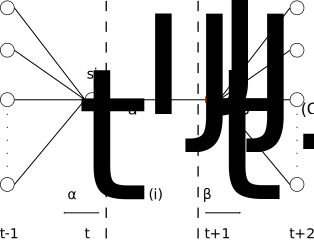
\includegraphics[height=0.35\textheight]{images/baum-welch-alg.pdf}
  	
\end{frame}
\subsection[Viterbi algorithm]{Uncovering Hidden states: Viterbi algorithm}
\label{sec:viterbi}

\begin{frame}
  \frametitle{Solve the best explanation problem}
  \begin{itemize}
  \item How can we answer the \emph{best explanation} problem?  \pause
  \item \textbf{Individually} most likely states
    \begin{equation}
      \label{eq:individually}
      \gamma_{t,i}=P(q_t = s_i \vert O, \lambda)
    \end{equation}
    \pause
  \item Computation
    \begin{equation}
      \label{eq:gamma_formula}
      \gamma_{t,i}=\frac{\alpha_{t,i}\beta_{t,i}}{P(O\vert \lambda)} =
      \frac{\alpha_{t,i}\beta_{t,i}}{\displaystyle\sum_{k=1}^{N}\alpha_{t,k}\beta_{t,k}}
    \end{equation}
    \pause
  \item Problems?
  \end{itemize}
\end{frame}

\begin{frame}
  \frametitle{Better optimality criterion}
  \begin{itemize}
  \item Can we find a better optimality criterion?  \pause
  \item Single best path \\
    $Q_{\text{best}} = [\hat{q}_1 \hat{q}_2 \cdots \hat{q}_T]$
    \begin{equation}
      Q_{\text{best}} = \underset{Q}{\operatorname{argmax}}\;
      P(Q \vert O, \lambda)
      = \underset{Q}{\operatorname{argmax}}\; P(Q, O \vert \lambda)
      \tag{\ref{eq:best-explanation}}
    \end{equation}
  \item \textbf{Viterbi algorithm} - dynamic programming
  \end{itemize}
\end{frame}

\begin{frame}
  \frametitle{$\delta$ variables}
  \begin{itemize}
  \item Introducing $\delta$ variables:
    \begin{equation}
      \label{eq:delta-definition}
      \delta_{t,i}=\underset{q_1,\ldots,q_{t-1}}{max} 
      P([q_1 q_2 \ldots q_{t-1} s_i], [o_1, o_2, \ldots o_t] \vert \lambda)
    \end{equation}
  \end{itemize}
  \begin{columns}
    \column{0.5\textwidth}
    \begin{itemize}
    \item $\delta_{t,i}$ - the highest probability for a sequence of
      $t$ states that ends in $s_i$ which accounts for the first $t$
      observations \visible<2>{
      \item the relation between \emph{sequential} $\delta$ variables:
        \begin{equation}
          \label{eq:delta-recurrence}
          \delta_{t,j} = [\underset{i}{max}\; \delta_{t-1,i} \cdot a_{i,j}] \cdot b_{j}(o_{t})
        \end{equation}}
    \end{itemize}
    \column{0.5\textwidth} \visible<2>{
      \includegraphics[width=\textwidth]{graphics/viterbi_path.pdf}
    }
  \end{columns}
\end{frame}

\begin{frame}
  \frametitle{Viterbi algorithm (I)}
  \begin{description}
  \item[1] Initialization: \\
    \begin{equation}
      \label{eq:viterbi-initialization}
      \begin{split}
        \delta_{1,i} & = \pi_{i}b_i(o_1), \quad 1 \le i \le N \\
        \psi_{1,i} & = 0
      \end{split}
    \end{equation}
  \item[2] Recursion: \\
    \begin{equation}
      \label{eq:viterbi-recursion}
      \begin{split}
        \delta_{t,j} & = [\underset{i }{max}\; \delta_{t-1,i} \cdot
        a_{i,j}] \cdot b_{j}(o_{t})
        \quad \scriptstyle{2 \le t \le T, 1 \le j \le N} \\
        \psi_{t,i} & = \underset{i}{argmax}\; \delta{t-1,i}\cdot
        a_{i,j} \quad \scriptstyle{2 \le t \le T, 1 \le j \le N}
      \end{split}
    \end{equation}
  \end{description}
\end{frame}

\begin{frame}
  \frametitle{Viterbi algorithm (II)}
  \begin{description}
  \item[3] Termination: \\
    \begin{equation}
      \label{eq:viterbi-termination}
      \begin{split}
        P(Q_{\text{best}} \vert O, \lambda) & = \underset{i}{max}\; \delta_{T,i} \\
        \hat{q}_T & = \underset{i}{argmax}\; \delta_{T,i}
      \end{split}
    \end{equation}
  \item[4] Backtracking: \\
    \begin{equation}
      \label{eq:viterbi-backtracking}
      \hat{q}_t = \psi_{t+1}(\hat{q}_{t+1}), \quad \scriptstyle{t=T-1,T-2,\cdots, 1}
    \end{equation}
  \end{description}
\end{frame}


\part{Demo \& Discussions}

\section{A Case for HMMs in Symbol Recognition}
\label{sec:sr}


\section{Types of HMMs}
\label{sec:types}


\section{Discussions and Recap}
\label{sec:final}

\begin{frame}
  \frametitle{Summary}
  \begin{itemize}
  \item HMM are useful for temporal sequence problems
    \pause
  \item there are 3 fundamental problems for HMMs:
    \begin{itemize}
    \item<3-> given an HMM, estimating the probability of an observed sequence
      \visible<6->{\structure{Forward-Backward Algorithm}}
    \item<4-> given observed data, estimating the parameters of an HMM
      \only<7->{\structure{Baum-Welch Algorithm}}
    \item<5-> uncovering the hidden states
      \visible<8->{\structure{Viterbi Algorithm}}
    \end{itemize}

  \end{itemize}
\end{frame}
\section[References]{}
\label{sec:references}
\begin{frame}[allowframebreaks]{References}
	\printbibliography
\end{frame}

\section[Thanks]{}
\label{sec:thanks}

\begin{frame}{Thank you!}
  
\end{frame}




\end{document}

